\documentclass[10pt,]{article}
\usepackage{lmodern}
\usepackage{amssymb,amsmath}
\usepackage{ifxetex,ifluatex}
\usepackage{fixltx2e} % provides \textsubscript
\ifnum 0\ifxetex 1\fi\ifluatex 1\fi=0 % if pdftex
  \usepackage[T1]{fontenc}
  \usepackage[utf8]{inputenc}
\else % if luatex or xelatex
  \ifxetex
    \usepackage{mathspec}
  \else
    \usepackage{fontspec}
  \fi
  \defaultfontfeatures{Ligatures=TeX,Scale=MatchLowercase}
\fi
% use upquote if available, for straight quotes in verbatim environments
\IfFileExists{upquote.sty}{\usepackage{upquote}}{}
% use microtype if available
\IfFileExists{microtype.sty}{%
\usepackage{microtype}
\UseMicrotypeSet[protrusion]{basicmath} % disable protrusion for tt fonts
}{}
\usepackage[margin=1in]{geometry}
\usepackage{hyperref}
\PassOptionsToPackage{usenames,dvipsnames}{color} % color is loaded by hyperref
\hypersetup{unicode=true,
            pdftitle={450 - Marketing Analytics - Solo 3},
            pdfauthor={R Sangole},
            colorlinks=true,
            linkcolor=Maroon,
            citecolor=Blue,
            urlcolor=blue,
            breaklinks=true}
\urlstyle{same}  % don't use monospace font for urls
\usepackage{graphicx,grffile}
\makeatletter
\def\maxwidth{\ifdim\Gin@nat@width>\linewidth\linewidth\else\Gin@nat@width\fi}
\def\maxheight{\ifdim\Gin@nat@height>\textheight\textheight\else\Gin@nat@height\fi}
\makeatother
% Scale images if necessary, so that they will not overflow the page
% margins by default, and it is still possible to overwrite the defaults
% using explicit options in \includegraphics[width, height, ...]{}
\setkeys{Gin}{width=\maxwidth,height=\maxheight,keepaspectratio}
\IfFileExists{parskip.sty}{%
\usepackage{parskip}
}{% else
\setlength{\parindent}{0pt}
\setlength{\parskip}{6pt plus 2pt minus 1pt}
}
\setlength{\emergencystretch}{3em}  % prevent overfull lines
\providecommand{\tightlist}{%
  \setlength{\itemsep}{0pt}\setlength{\parskip}{0pt}}
\setcounter{secnumdepth}{0}
% Redefines (sub)paragraphs to behave more like sections
\ifx\paragraph\undefined\else
\let\oldparagraph\paragraph
\renewcommand{\paragraph}[1]{\oldparagraph{#1}\mbox{}}
\fi
\ifx\subparagraph\undefined\else
\let\oldsubparagraph\subparagraph
\renewcommand{\subparagraph}[1]{\oldsubparagraph{#1}\mbox{}}
\fi

%%% Use protect on footnotes to avoid problems with footnotes in titles
\let\rmarkdownfootnote\footnote%
\def\footnote{\protect\rmarkdownfootnote}

%%% Change title format to be more compact
\usepackage{titling}

% Create subtitle command for use in maketitle
\newcommand{\subtitle}[1]{
  \posttitle{
    \begin{center}\large#1\end{center}
    }
}

\setlength{\droptitle}{-2em}

  \title{450 - Marketing Analytics - Solo 3}
    \pretitle{\vspace{\droptitle}\centering\huge}
  \posttitle{\par}
    \author{R Sangole}
    \preauthor{\centering\large\emph}
  \postauthor{\par}
    \date{}
    \predate{}\postdate{}
  

\begin{document}
\maketitle

\section{Methodology Discussion}\label{methodology-discussion}

The input data for this modeling exercise is a combination of aggregated
customer transaction history data, customer profile information,
customer preference information and also demographic data for each
zipcodes. The input data is large dataset (30779 rows, each for an
individual customer) and 554 variables (numerical and categorical
combined).

\section{Data Preparation}\label{data-preparation}

The data required significant pre-preparation before modeling could be
done. To summarize the data preparation steps taken:

\begin{itemize}
\tightlist
\item
  Factor variables with \texttt{NA} and \texttt{U} (Unknown) levels are
  both re-labeled at \texttt{U}
\item
  Numerical variables originally as characters or factors are typecasted
  appropriately
\item
  Factor variables with either very large number of levels, or with
  certain levels contributing to very small percentage of the overall
  data (1\% or less) are re-leveled, i.e.~levels with very small number
  of variables are grouped together into \texttt{Other}
\item
  Variables with near zero variance are removed. These are identified
  using the \texttt{caret::nearZeroVar()} call. Fully zero variance
  calls are also removed using this function.
\item
  New variables are created based on the originals. Brief description

  \begin{itemize}
  \tightlist
  \item
    cusum\_resp\_till15 : How many times has the customer responded in
    the past, till campaign 15?
  \item
    cusum\_qty\_till15 : How much has the customer purchased in the
    past, till campaign 15?
  \item
    cusum\_tot\_usd\_till15 : How much has the customer spent in the
    past, till campaign 15?
  \item
    cusum\_tot\_usd\_12\_to\_15 : How much has the customer spent in the
    past, from campaign 12 to campaign 15?
  \item
    old\_response\_15 : Binary variable (0/1) indicating if the customer
    reponded for the old campaign
  \item
    old\_response\_14 : Binary variable (0/1) indicating if the customer
    reponded for the old campaign
  \item
    old\_response\_13 : Binary variable (0/1) indicating if the customer
    reponded for the old campaign
  \item
    old\_response\_12 : Binary variable (0/1) indicating if the customer
    reponded for the old campaign
  \item
    old\_response\_11 : Binary variable (0/1) indicating if the customer
    reponded for the old campaign
  \item
    cusum\_mailers\_till15 : Total mailers till campaign 15
  \item
    mailers\_in\_15 : Mailers mailed in recent past, campaign 15
  \item
    mailers\_in\_14 : Mailers mailed in recent past, campaign 14
  \item
    PRE2009\_SALES : Life-To-Date sales - Year-To-Date-2009 sales
  \item
    PRE2009\_TRANSACTIONS : Life-To-Date transactions -
    Year-To-Date-2009 transactions
  \end{itemize}
\end{itemize}

\subsection{Imputation}\label{imputation}

There are many variables with missing values in the original dataset.
Depending on the nature of the model, NA values may or may not be
acceptable. To counter the \texttt{NA} values in the dataset, two
approaches were taken, at a high level:

\begin{enumerate}
\def\labelenumi{\arabic{enumi}.}
\tightlist
\item
  For numeric variables, the random forest approach in the \texttt{mice}
  package is used, with a repeated imputation of \texttt{m=5}. The
  resulting imputation densities are very close to the original
  densities. Refer to \protect\hyperlink{impute_num}{figure}. A
  comparison of the blue and red curves show similar curves.
\item
  For categorical variables, a similar approach was attempted. Various
  techniques (randomforest, pmm, cart or mean) were attempted, however,
  I was not succesful in completing this imputation, due to memory \&
  computation constraints of the machine I have. As a result, to
  simplify the computation, I have two strategies:
\end{enumerate}

\begin{itemize}
\tightlist
\item
  For levels which contain ``U'' or ``Unknown'', the \texttt{NA} are
  recoded to ``U''
\item
  For levels which do not contain ``U'', \texttt{NA} are recoded to
  ``U''
\end{itemize}

\subsection{Data Splits}\label{data-splits}

There are two types of data splits conducted:

\begin{enumerate}
\def\labelenumi{\arabic{enumi}.}
\item
  Train + Test Split for Modeling
\item
  Train + Calibration + Test for Variable Selection
\end{enumerate}

\subsection{Initial Variable
Selection}\label{initial-variable-selection}

\section{Model Approach}\label{model-approach}

\subsection{Random Forests}\label{random-forests}

\subsection{SVM}\label{svm}

\subsection{Deepboosting}\label{deepboosting}

\section{Modeling Results}\label{modeling-results}

Interpreting the average values in
\protect\hyperlink{overall_beta_table}{table 2}, we can see that:

\section{Final Recommendation to STC}\label{final-recommendation-to-stc}

\newpage

\section{Appendix}\label{appendix}

\hypertarget{impute_num}{\paragraph{Numerical variables imputation
results}\label{impute_num}}

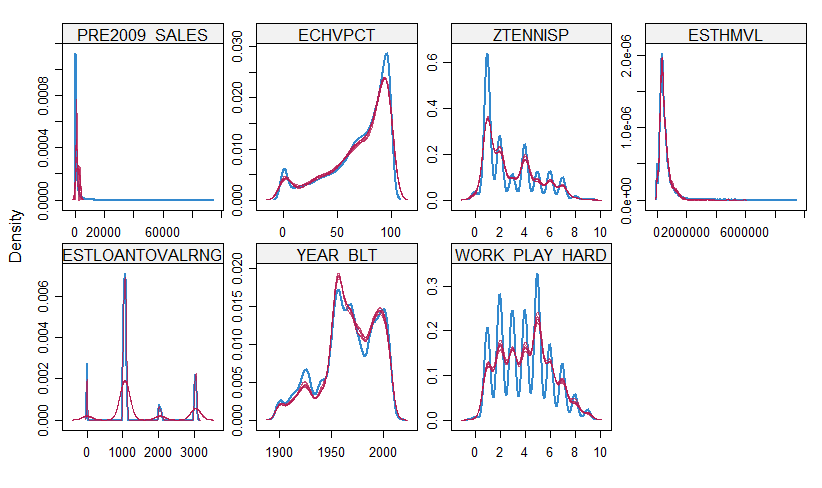
\includegraphics[width=0.8\linewidth]{images/report_mice_num}

\newpage

\section{Code}\label{code}


\end{document}
